\documentclass{standalone}
\usepackage{tikz}
\begin{document}
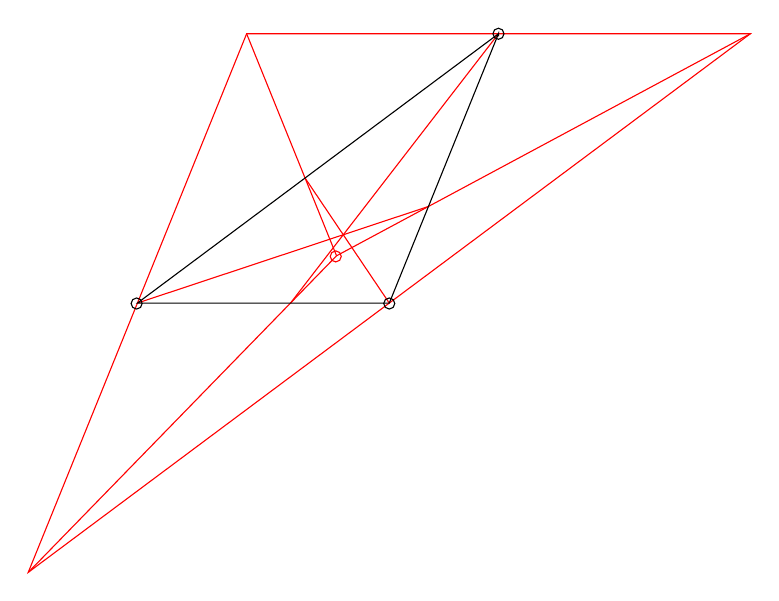
\begin{tikzpicture}[x=1pt,y=1pt]
\draw[red] (16.53,-215.53) -- (95.45,-20.90) -- (277.46,-20.90) -- cycle;
\draw[red] (186.45,-20.90) -- (111.30,-118.22);
\draw[red] (55.99,-118.21) -- (161.15,-83.31);
\draw[red] (146.99,-118.21) -- (116.56,-73.02);
\draw[red] (277.46,-20.90) -- (127.94,-101.13);
\draw[red] (95.45,-20.90) -- (127.94,-101.13);
\draw[red] (16.53,-215.53) -- (127.94,-101.13);
\draw[red] (127.65,-101.35) circle (2.00);
\draw (186.45,-20.90) -- (55.99,-118.21) -- (147.00,-118.21) -- (186.45,-20.89) -- (186.45,-20.89) -- (186.45,-21.80) -- cycle;
\draw (186.45,-20.90) circle (2.00);
\draw (55.70,-118.37) circle (2.00);
\draw (146.99,-118.37) circle (2.00);
\end{tikzpicture}
\end{document}
